\documentclass{article}
\usepackage{hyperref}
\usepackage{listings}
\usepackage{graphicx}

\title{LoFASM Pulsar Search with PRESTO}
\author{Keith E. Boehler Jr.}
\date{}
\begin{document}
   \maketitle
   Hello world!
   
   \section{Installing Presto}
   The instructions here are based on those by Scott Ransom's Install page on github as well as other 
   tips found on the internet. The following will be centered on using Ubuntu 20.04. Tips for macOS Mojave
   will be provided as well. 
   
   \subsection{FFTW 3}
    This one is rather straight forward. 
    \begin{enumerate}
    	\item At the time of this writing the latest version is 3.3.8 and can be downloaded \href{http://www.fftw.org/download.html}{from this link}
    	\item \noindent Once the source has been downloaded it can be unpacked using the command:
	    \begin{lstlisting}[language=bash]
	    $ tar -zx fftw-x.x.x.tar.gz 
	    \end{lstlisting}
    	(Will need to replace the x.x.x with the current version number). And enter the unpacked directory.
    	\item \noindent After that we need to configure. According to Scott there are some suggested flags if you are
    	using an Intel chip, which I am. So my command will look like: 
	    \begin{lstlisting}[language=bash]
	    ./configure --prefix=$HOME \
	    --enable-shared --enable-single \
	    --enable-sse --enable-sse2 --enable-avx \
	    --enable-avx2 --enable-fma
	    \end{lstlisting}
	    \item \noindent Followed by: \begin{lstlisting}[language=bash]
	    $ make
	    \end{lstlisting}
	    \item \noindent Followed by: 
		\begin{lstlisting}[language=bash]
		$ make check
		\end{lstlisting}
	    \item \noindent Followed by: 
		\begin{lstlisting}[language=bash]
		$ make install
		\end{lstlisting}
	    \item \noindent Followed by:
		\begin{lstlisting}[language=bash]
		 $ make installcheck
		\end{lstlisting}
    	\end{enumerate}
    	Due to the fact that we used \$HOME in our prefix we should have /bin /include and other directories
    	being made in our home directory. This will help later when we are making our environment variables
    	as the location of configure files and executable will be in more standard location.
    
    	\subsection{PGPLOT}
    	This one is a bit involved, so I recommend brewing your favorite cup of Joe before getting started. This
    	portion is based on the PGPLOT’s instructions for all UNIX systems. 
    	\begin{enumerate}
    	\item \noindent I downloaded my source for PGPlot from \href{ftp://ftp.astro.caltech.edu/pub/pgplot/pgplot5.2.tar.gz}{here, version 5.2.}. And untarred with: 
    	\begin{lstlisting}[language=bash]
    	$ tar -xzvf pgplot5.2.tar.gz
    	\end{lstlisting}
    	 At this point it is prudent to create what the pgplot unix instructions call the target directory, that is where we will install. I find it to be clear to rename the directory we just unpacked to \texttt{pgplot\_src} and the actual install directory to be \texttt{pgplot}. 
    	\item Copy the drivers list from the source directory (\texttt{pgplot\_src}) into our install directory (\texttt{pgplot}). If you are inside the install directory here is a snippet: \noindent
    	\begin{lstlisting}[language=bash]
    	$ cp ../pgplot_src/drivers.list .
    	\end{lstlisting} 
    	\item Using any text editor open the drivers file. Uncomment the needed drivers by removing the `` ! '' from the needed line. It is recommended to only uncomment the needed drivers. For PRESTO we at a minimum need the postscript (those with PS in the name) and xwindow (xw and xserver). And save the changes. 
    	\item Create the Makefile. This step can be somewhat involved so a fresh pot of coffee is needed to lift spirits. While the below is going to be centered for Ubuntu 20.04 I do have some tips for installing on macOS Mojave. I used homebrew to install xquartz (an xserver for mac), gcc (for gfortran and the c compiler.), and there is also a special configuration file that can be found \href{http://mingus.as.arizona.edu/~bjw/software/pgplot_macosx_conf.tar}{at this location}. Otherwise the following should be similar:
    		\begin{enumerate}
    			\item Run the makemake script with the following template: \texttt{path2/pgsrc/makemake path2/pgsrc Ostype fortran/cc}. That is to say while in your target directory run stuff in your source directory. Select if you are using linux and a C-Compiler and Fortran compiler. It is worth noting that we will edit the resulting Makefile with the compilers we will actually use. My command looks like this: \begin{lstlisting}[language=bash]

$./pgplot_src/makemake ../pgplot_src/ linux g77_gcc
    			\end{lstlisting}
    			\item Enter the makefile and change the \texttt{FCOMPL} to \texttt{gfortran} (install if you dont have it at this point. Also on macOS should change the C compiler to a gcc one). Then type \texttt{make}. My install of Ubuntu is fresh so it was also missing \texttt{libx11-dev} (X11/Xos.h: No such file or directory ← Error). Here is what a successful run looks like: Figure \ref{fig:pgplot-make}.     			
    			\begin{figure}[h]
    				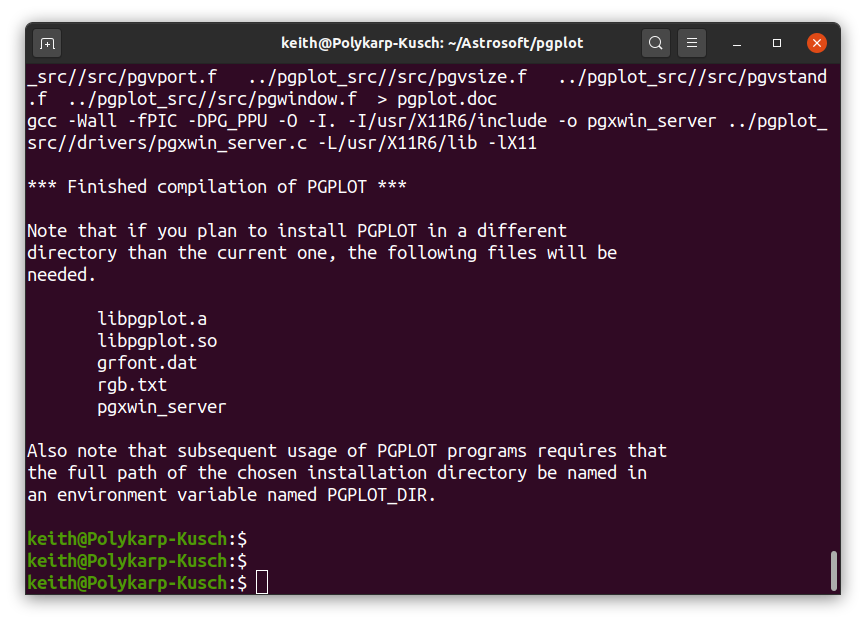
\includegraphics[width=\linewidth]{Images/sucesfful-pgplot-make.png}
    				\caption{Successful PGPlot make}
    				\label{fig:pgplot-make}  			
    			\end{figure}
    			\item Enter: \texttt{\$ make cgp} \ref{fig:pgplot-make-cpg}
    			\begin{figure}[h]
    				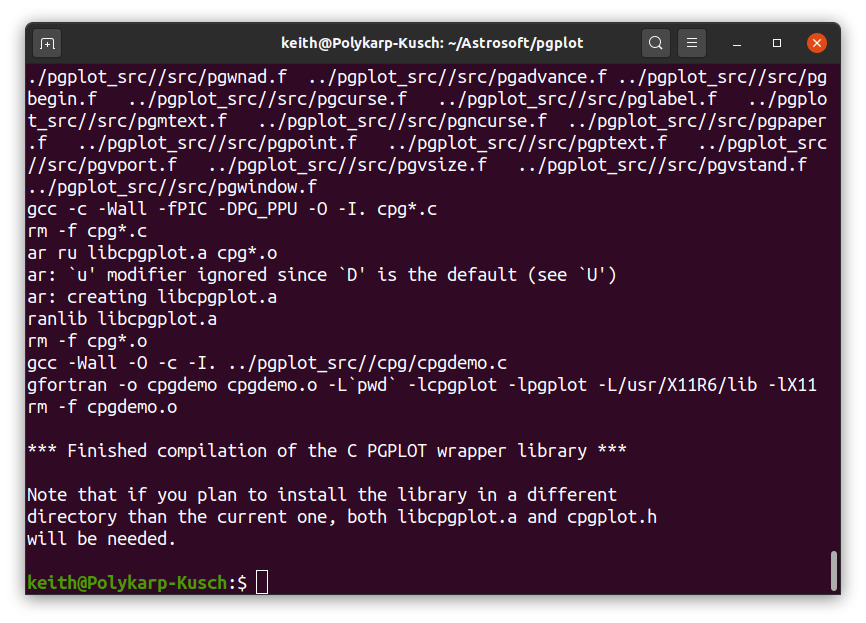
\includegraphics[width=\linewidth]{Images/sucesfful-pgplot-make-cgp.png}
    				\caption{Successful PGPlot make cpg}
    				\label{fig:pgplot-make-cpg}  			
    			\end{figure}
    			\item Enter: \texttt{\$ ld -shared -o libcpgplot.so --whole-archive libcpgplot.a}
    			
    			
    			\item At this point we should set our environment variables 
    			\footnote{I like to keep a file in my home directory called \texttt{.bash\_astro}. In it i have a variable called \texttt{ASTROSOFT} that points to where i am installing my programs. For example my \texttt{LD\_LIBRARY\_PATH} will be defined as: \texttt{export LD\_LIBRARY\_PATH=\$ASTROSOFT/pgplot:\$LD\_LIBRARY\_PATH}. The word \texttt{export} tells bash this is environment variable. The \texttt{\$} is used to envoke other variables. The \texttt{':'} is to re-appending any previous \texttt{LD\_LIBRARY\_PATH}.}. 
    			This will allow our shell to find shared objects, executables, and device outputs. We will need the \texttt{PGPLOT\_DIR=/path/to/pgplot}; this should have the files \texttt{grfont.dat} and \texttt{rgb.txt}. We will also need a \texttt{LD\_LIBRARY\_PATH} that should point to the file \texttt{libpgplot.so}, If you compiled from source like we did in this example it should be in the same big directory. Finally we can set the \texttt{PGPLOT\_DEV=/XWINDOW} to default to outputting to an xwindow. 
    			
    			\item In principle we are done. Now lets test our work by running the demo programs \ref{fig:sucesfful-pgplot-install}.  
    			\begin{figure}[h]
    				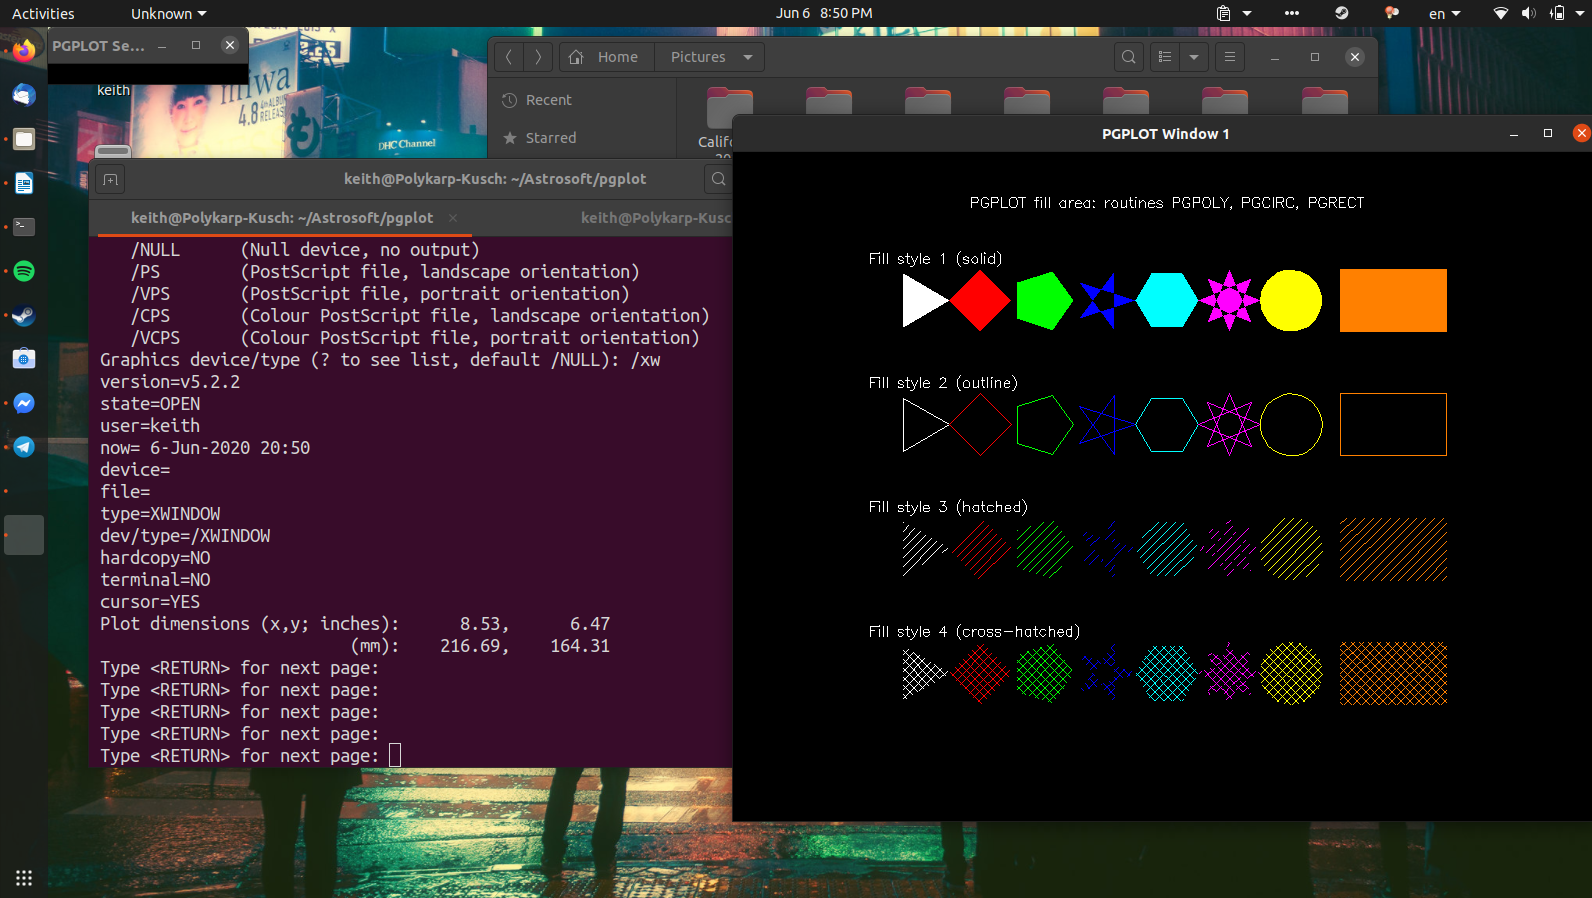
\includegraphics[width=\linewidth]{Images/sucesfful-pgplot-install.png}
    				\caption{Run them with ./pgdemo1}
    				\label{fig:sucesfful-pgplot-install}  			
    			\end{figure}    	
    		\end{enumerate}   		
    	\end{enumerate}
    	
    	\subsection{TEMPO}
    	\begin{enumerate}
    		\item Cloning the source from \href{git://git.code.sf.net/p/tempo/tempo}{git.} 
    	\end{enumerate}

    	
\end{document} 
